\section{ELMo} \label{sec:ELMo}


\subsection{Combing Back To Polysemy} \label{sec:PolysemyAgainInElmo} 

As explained in \nameref{sec:ProblemWithStaticEmbs}, the term \textbf{\hyperref[sec:Polysemy]{polysemy}} is the correspondence of one word to distinct meanings, and traditional embeddings fail to capture these senses, thus performing poorly on language modeling NLP tasks. However \hyperref[sec:SolutionWithContextEmbs]{contextual embeddings (CWE)} prove superior since they create one vector representation for each word type in the vocabulary and also create distinct word vectors per token given a context (Wiedemann et al., 2019). For instance, relying on word and character embedding alone, a pair of homonyms like ``book," as in a text or literature, and ``book", as in to make a reservation, would be assigned the same vector representation even though these are different words. This vector representation might include context, as per the \nameref{sec:Word2Vec} or \nameref{sec:Glove}, but these meanings are collapsed into a single representation, so the vector's meaning would be change depending on its training data. 


\subsection{Motivation for ELMo} 


In contrast to traditional word embeddings, \textbf{deep contextualized word embeddings} from Peters et al. (2018) capture word semantics in context to account for the context-dependent and polysemous nature of words. These word vectors are ``learned functions of the internal states of a \hyperref[sec:BidirectionalLM]{bidirectional language model (biLM)}" that is pretrained on a large corpus. For this reason, the resulting word representations are called \textbf{ELMo (Embeddings from Language Models)} and they can be mixed into existing models. 

According to Peters at al. (2018), \textbf{ELMo representations} are \emph{deep} since they are a function of all internal layers of the biLM. ELMo learns a ``linear combination of vectors stacked above each input word for each end task" which improves performance over models simply using the top \hyperref[sec:LSTM]{LSTM} layer. This results in richer word representations since higher-level LSTM layers capture contextual meaning, useful for supervised word sense disambiguation (WSD), while lower layers capture syntax information, useful for part-of-speech tagging (POS). 

``Simultaneously exposing all of these signals is highly beneficial, allowing the learned models to select the types of semi-supervision that are most useful for each end task" (Peters et al., 2018). 


\subsection{Describing ELMo} 

``ELMo is a task specific combination of the intermediate layer representations in the biLM" (Peters et al., 2018). 

Formally, for each word token $t_k$, an $L$-layer bidirectional language model creates $2L + 1$ representations: 

$$
\begin{array}{ll}
R_k 
&= \Big \{ \mathbf{x}_k^{LM}, \; \overrightarrow{\mathbf{h}}_{kj}^{LM}, \; \overleftarrow{\mathbf{h}}_{kj}^{LM} \; | \; j = 1,...,L \Big \} \\
&= \Big \{ \mathbf{h}_{kj}^{LM} \; | \; j = 1,...,L \Big \}
\end{array}
$$
where $\mathbf{h}_{k0}^{LM}$ is the token layer and the hidden state vector $\mathbf{h}_{kj}^{LM} = \Big \{ \overrightarrow{\mathbf{h}}_{kj}^{LM}, \; \overleftarrow{\mathbf{h}}_{kj}^{LM}  \}$, a concatenation of backward and forward hidden states, for each bidirectional LSTM layer. 

ELMo collapses all layers in the above vector into a single vector to create an ELMo word embedding ready for immediate application in an NLP task. ELMo does this by weighting the biLM layers in a task-specific way (Peters et al., 2018): 
$$
\textbf{ELMo}_k^{task} = E \Big( R_k; \theta^{task} \Big) = \gamma^{task} \; \sum_{j=0}^L s_j^{task} \; \mathbf{h}_{kj}^{LM}
$$
where the vector $\mathbf{s}^{task} = \Big\{ s_j^{task} \Big\}$ of softmax-normalized weights and task-dependent scalar parameter $\gamma^{task}$ allow the model for the specific $task$ to scale the entire $\textbf{ELMo}_k^{task}$ vector. The index $k$ corresponds to a $k$-th word, and index $j$ corresponds to the $j$-th layer out of $L$ layers. Specifically, $h_{kj}^{LM}$ is the output of the $j$-th LSTM for word $k$, and $s_j$ is the weight of $h_{kj}^{LM}$ used to compute the representation for word $k$. 

The bidirectional language model component of ELMo is task-agnostic, and ELMo combines the task-independent representations. Although the hidden states are fixed, this ELMo formulation is flexible enough to be combined in downstream models for various tasks (Kurita, 2018b). 

ELMo can be applied to specific tasks by concatenating the ELMo word embeddings with context-free word embeddings, such as those from GloVe, FastText, or character embeddings. From Peters et al. (2018), the concatenated input vector $\Big\{ \mathbf{x}_k \; ; \; \textbf{ELMo}_k^{task} \Big\}$ would be passed into a task-specific RNN for processing. Additionally, authors found that for question answering (QA), concatening ELMo embeddings with outputs of the question answering model could improve performance. 

\subsection{ELMo Experimental Results} \label{sec:ResultsELMo}

\begin{itemize}
    \item  \textbf{Question answering (QA): } Peters et al. (2018) added ELMo embeddings to a baseline biLM model with attention from Seo et al. (2017) and found this improved the test set $F_1$ score of the biLM model from $81.1 \%$ to $85.8 \%$, a state-of-the-art result. 

    \item \textbf{Semantic role labeling (SRL): } When adding ELMo representations to an 8-layer deep biLSTM that interwove forward and backward directions, the single test set $F_1$ score increased by $3.2 \%$, which is a $1.2 \%$ improvement over the previous best model. 
    
    \item \textbf{Coreference resolution (CR): } Using Lee et al. (2017)'s model that uses attention to compute span vectors transformed by softmax ranking to find coreference chains, adding ELMo embeddings improved the average $F_1$ score by $3.2 \%$, improving over the previous best model by nearly two percentage points. 
    
    \item \textbf{Named entity extraction (NER): } The baseline model had pretrained, character embeddings from a convolutional neural network (CNN), as well as two biLSTM layers and a conditional random field (CRF) loss function formulation (Lafferty et al., 2001). Adding ELMo embeddings $92.22 \%$ in $F_1$ score by letting the task model learn an average of all biLM layers, rather than only using the top layer. 
    
    \item \textbf{Sentiment analysis (SA): } A classification model using contextual embeddings from the CoVe model (McCann et al., 2018) was used as the baseline model, with CoVe embeddings replaced by ELMo embeddings. This resulted in a full percentage increase in absolute accuracy over state of the art. 
\end{itemize}


\subsection{ELMo's Defining Success} \label{sec:ELMoSuccessFeature}

ELMo's biLM captures meaning differently; lower layers are better for representing syntactic meaning, while higher layers capture semantic information. Because ELMo improves task performance over word embeddings, this must mean its biLM's contextual representation outputs are encoding task-specific information that traditional word vectors do not otherwise capture. In other words, the biLM must be sifting meaning of words using their context. 


\begin{table}[ht!]
  \centering
  \begin{tabular}{ c }
    
    \begin{minipage}{.8\textwidth}
      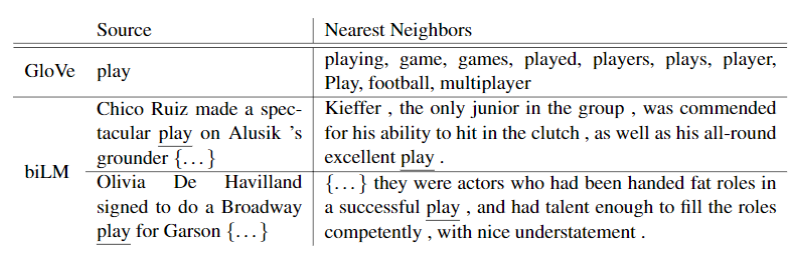
\includegraphics[width=\linewidth]{imgs/table_elmoPlay.png}
    \end{minipage}
    
  \end{tabular}
  \caption{\footnotesize Nearest neighbors to ``play” using GloVe and the context embeddings from a biLM. From \emph{Table 4 in Deep Contextualized Word Representations}, by Peters et al., 2018. \url{https://arxiv.org/pdf/1802.05365.pdf}. Copyright 2018 by Peters et al.}
  \label{tbl:elmoPlayExample}
\end{table}


The word ``play" is highly polysemous since it has many different meanings.  \cref{tbl:elmoPlayExample} displays words nearest to ``play" found using GloVe word embeddings and a biLM model. The GloVe's neighbors include several different parts of speech, like verbs (``played", ``playing), and nouns (``player", ``game") and only in the sport sense of the word. However, the bottom two rows show that the nearest neighbor sentences from the biLM's contextual embedding of ``play" can disambiguate between \emph{both} the parts of speech \emph{and} word sense of ``play". The last row's input sentence contains the noun / acting sense of ``play" and this is matched in the nearest neighbor sentence, highlighting ELMo's strength in \textbf{part of speech tagging (POS)} and \textbf{word sense disambiguation (WSD)}. 